%  LaTeX support: latex@mdpi.com
%  manuscriptR1V2.tex: Round-1 revision rewrite.
%  Based on the MDPI Mathematics template from first_round/.
%  Internal bibliography (MDPI ACS format): references are embedded below;
%  biblio.bib is the editable source. To refresh after citation changes:
%  temporarily use \bibliography{biblio}, run pdflatex+bibtex, and copy the .bbl.

%=================================================================
\documentclass[mathematics,article,submit,moreauthors]{Definitions/mdpi}

%=================================================================
% MDPI internal commands - do not modify
\firstpage{1}
\makeatletter
\setcounter{page}{\@firstpage}
\makeatother 
\pubvolume{1}
\issuenum{1}
\articlenumber{0}
\pubyear{2026}
\copyrightyear{2026}
%\externaleditor{Firstname Lastname}
\datereceived{ }
\daterevised{ }
\dateaccepted{ }
\datepublished{ }

%=================================================================
\usepackage{xcolor}

%=================================================================
% Full title of the paper (Capitalized)

\Title{Aggregation Semantics for Prioritization in Cooperative Automated Decision Making}

% Author Orchid ID: enter ID or remove command
\newcommand{\orcidauthorA}{0000-0003-3267-6753}
\newcommand{\orcidauthorB}{0009-0002-0183-7905}
\newcommand{\orcidauthorC}{0000-0002-7653-1452}

% Authors, for the paper (add full first names)
\Author{Pavel Novoa-Hern\'andez$^{1,*}$\orcidA{}, Mariia Godz$^{2}$\orcidA{} and David A. Pelta$^{2}$\orcidC{}}

% MDPI internal command: Authors, for metadata in PDF
\AuthorNames{Pavel Novoa-Hern\'andez, Mariia Godz and David A. Pelta}

% Affiliations / Addresses
\address{%
$^{1}$ \quad Dept. Computer Engineering and Systems, Universidad de La Laguna; pnovoahe@ull.edu.es\\
$^{2}$ \quad Dept. Computer Science and Artificial Intelligence, Universidad de Granada; \{mariiagodz,dpelta\}@ugr.es}

% Contact information of the corresponding author
\corres{Correspondence: pnovoahe@ull.edu.es}

% Abstract placeholder (to be rewritten with the new structure)
\abstract{To be rewritten.}

% Keywords
\keyword{
cooperative automated decision making;
aggregation operators;
multi-criteria decision making;
context-aware decision support;
prioritization
}

%%%%%%%%%%%%%%%%%%%%%%%%%%%%%%%%%%%%%%%%%%
\begin{document}

% ==============================================================================
% NOTA GLOBAL DE ESTILO:
% [Aborda 2.8 y M1.7]: Todo el documento debe ser reescrito en tercera persona
% (evitar "We provide", "We compare") y con una revisi\'on exhaustiva de ingl\'es.
% ==============================================================================

\section{Introduction}

% R1-1, R2-2
% Posicionar claramente la novedad.
% No proponemos un nuevo operador ni un nuevo método fuzzy MCDM.
% La contribución es metodológica: estudiar la agregación como mecanismo
% de gobernanza dentro de una arquitectura cooperativa ADM.

% R2-3
% Introducir explícitamente los research questions (RQ1-RQ4).

% R2-4
% Al final de la sección incluir la tabla cronológica de literatura
% (o referenciarla si se coloca en Background).

% R1-12, R2-6
% Justificar desde el principio por qué se estudian tres regímenes:
% compensatorio, parcialmente compensatorio y no compensatorio.

\subsection{Research Questions and Contributions}

% R2-3
% Formular RQ1-RQ4.
% Enumerar contribuciones metodológicas y experimentales.

%%%%%%%%%%%%%%%%%%%%%%%%%%%%%%%%%%%%%%%%%%%%%%%%%%%%%%%%%%%%

\section{Background and Related Work}

% R1-1, R2-2, R2-3, R2-4
% Construir el gap de investigación.
% Distinguir explícitamente el trabajo de:
% - fuzzy MCDM,
% - aggregation theory,
% - context-aware DSS, 
% - cooperative ADM. 

\subsection{Context-Aware and Cooperative Decision Support Systems}
\label{subsec:context-aware-dss}
% R2-2, R2-3
% Revisar Teng, Yao, Cronholm, Merkert, etc.
% Mostrar que el foco suele estar en reglas, ontologías o interacción.

The increasing adoption of Artificial Intelligence (AI) in decision-support systems has highlighted the need to complement predictive performance with contextual, organizational, and domain-specific knowledge. In many real-world settings, decisions cannot be based solely on statistical predictions because institutional policies, expert knowledge, regulatory requirements, and operational constraints must also be considered. As a result, a growing body of research has focused on context-aware and cooperative decision-support systems capable of integrating heterogeneous sources of information into the decision-making process.

One important research direction concerns the incorporation of explicit knowledge representations alongside data-driven models. Early examples include cognitive-agent architectures that combine symbolic rules with machine-learning mechanisms to support context-aware decision making \citep{TengTan2008}. Similarly, ontology-based clinical decision-support systems have employed contextual ontologies and clinical pathways to select context-appropriate recommendations for individual cases \citep{YaoKumar2012}. More recent developments have extended these ideas through semantic models, knowledge graphs, and hybrid AI architectures that combine predictive models with structured domain knowledge to improve decision quality and interpretability \citep{AbuRasheed2024,Casado2025Governance}.

A second research stream emphasizes cooperation between human and artificial intelligence. Rather than viewing decision support as a purely predictive task, these approaches consider decision making as a collaborative process in which machine-learning models provide evidence while human experts contribute contextual understanding, oversight, and governance. Cronholm and G\"obel \citep{CronholmGoebel2022}, for example, argue that effective decision support requires appropriate mechanisms for combining human and artificial intelligence rather than simply improving predictive accuracy. Likewise, recent surveys on human-centred AI highlight transparency, accountability, contextual awareness, and governance as fundamental requirements for trustworthy decision-support systems \citep{Fanfani2025Human}.

Related ideas also appear in cooperative and distributed decision-making environments. Multi-agent systems, collective-intelligence frameworks, and cooperative AI architectures frequently rely on multiple decision sources that must be reconciled before a final recommendation is produced \citep{Smirnov2021Methodology}. In these settings, contextual information often plays a coordinating role by constraining, guiding, or validating the outputs generated by predictive components. Similar concerns arise in governance-oriented decision-support systems, where contextual information may encode operational procedures, organizational priorities, safety requirements, or regulatory obligations \citep{Marot2022Perspectives,Casado2025Governance}.

Taken together, these studies clearly demonstrate the importance of
contextual knowledge in decision-support systems. However, their primary
focus typically lies in knowledge representation, ontology design,
human--AI interaction, governance mechanisms, or system architecture.
Once predictive evidence and contextual assessments have been generated,
the numerical integration process that combines both sources of
information is often treated as a secondary implementation detail.
Consequently, relatively little attention has been devoted to
understanding how alternative integration mechanisms affect the final
recommendations produced by the system.

This limitation becomes particularly visible in architectures that
explicitly separate predictive evidence from contextual assessment.
Recent work on Cooperative Automated Decision-Making Systems (CADEMAS)
\citep{NovoaHernandez2026} and its machine-learning instantiation
CADEMAS-ML \citep{Godz2026} exemplifies this design philosophy.
CADEMAS organizes heterogeneous automated decision-making components and
contextual knowledge into distinct layers, allowing predictive evidence
and contextual assessments to be generated independently before being
combined into a final recommendation. Such architectures make the
integration mechanism itself an explicit design choice rather than an
implicit implementation detail. As a result, the aggregation operator
determines how predictive evidence interacts with contextual
requirements, organizational priorities, or policy constraints, thereby
shaping the semantics of the resulting decision process.

This observation suggests that aggregation should not be viewed merely
as a numerical post-processing step. Instead, it can be interpreted as a
governance mechanism that regulates the interaction between predictive
and contextual information. Understanding the implications of different
aggregation semantics therefore becomes essential for the design of
cooperative and context-aware decision-support systems. The next
subsection reviews the aggregation literature from this perspective. 

\subsection{Aggregation Operators and Decision Semantics}
\label{subsec:aggregation-operators-and-decision-semantics}

% R1-1, R1-12, R2-2, R2-6
% Revisar OWA, t-norms, geometric operators, consensus aggregation.
% Introducir la idea de compensación.

Aggregation operators constitute one of the central building blocks of
multi-criteria decision making (MCDM), fuzzy decision support, and
collective decision-making systems. Their purpose is to combine multiple
sources of information into a single assessment while preserving, to a
greater or lesser extent, the decision semantics associated with the
original criteria. Consequently, aggregation has been studied
extensively from both theoretical and applied perspectives.

Among the most influential aggregation frameworks are Ordered Weighted
Averaging (OWA) operators \citep{Yager1988,Yager2005}, t-norm and
t-conorm based operators, geometric aggregation functions, and
non-additive integrals such as the Choquet and Sugeno integrals.
Collectively, these approaches provide a rich mathematical vocabulary
for representing different attitudes toward compensation, conjunction,
disjunction, and interaction among criteria. From this perspective, the
choice of aggregation operator is not merely a numerical convenience but
a modeling decision that determines how favorable and unfavorable
evidence may compensate for one another.

A substantial body of literature has explored these properties in
traditional decision-making settings. Reviews by
Mardani et al.~\citep{Mardani2018} and
Csisz\'ar~\citep{Csiszar2021} highlight the widespread use of OWA-based
aggregation and related fuzzy operators across diverse application
domains. More recent studies have continued to investigate how
aggregation semantics influence consensus formation, robustness,
criterion interaction, and ranking behavior. Examples include
consensus-oriented aggregation in group decision making
\citep{MoralEtAl2017,TrilloEtAl2023}, robust Choquet-based decision
models \citep{Yang2022Tolerance,Liao2023Contextual}, and applications
employing geometric and OWA-type operators to capture alternative
decision attitudes \citep{Stroppiana2022Explainable,Alcantud2023Multi}.

Despite this methodological richness, most aggregation studies are
formulated within classical MCDM settings, where the aggregated inputs
represent multiple criteria, attributes, preferences, or expert
judgments associated with the same decision problem. The primary
objective is typically to identify the most appropriate operator for
combining these criteria or to develop new aggregation mechanisms with
desirable mathematical properties. Comparatively less attention has been
paid to architectures in which the aggregated inputs originate from
fundamentally different decision layers.

This distinction is particularly important in cooperative automated
decision-making systems. In architectures such as CADEMAS-ML, the
aggregation process does not combine multiple criteria describing an
alternative. Instead, it reconciles two conceptually distinct sources of
evidence: a predictive assessment generated by machine-learning models
and a contextual assessment encoding organizational priorities,
regulatory requirements, expert knowledge, or policy constraints. Under
this interpretation, the aggregation operator effectively determines the
extent to which predictive evidence may compensate for weak contextual
support, or conversely, whether contextual constraints can restrict
otherwise favorable predictions. The operator therefore acts as an
implicit governance mechanism rather than merely a criterion-combination
tool.

For this reason, the present work focuses on three representative
aggregation regimes exhibiting fundamentally different compensation
semantics. The weighted arithmetic mean represents a fully compensatory
integration strategy in which predictive and contextual information may
offset one another. The weighted geometric mean represents a partially
compensatory strategy that penalizes strong imbalances between both
sources of evidence. Finally, the minimum operator represents a
non-compensatory strategy in which the weakest component determines the
final assessment. Together, these operators span a spectrum ranging from
highly permissive to highly restrictive integration behavior while
remaining interpretable and widely understood within the aggregation
literature.

From the perspective of this study, the objective is therefore not to
propose a new aggregation operator nor to extend aggregation theory.
Instead, aggregation operators are treated as alternative decision
semantics within a cooperative automated decision-making architecture.
The key question is how different compensation regimes influence policy
compliance, prioritization behavior, robustness to predictive
perturbations, and ranking stability when predictive and contextual
information must jointly determine the final recommendation.

\subsection{Research Gap and Positioning}
\label{subsec:research-gap}
% R1-1, R2-2, R2-3
% Diferenciar explícitamente la contribución respecto a:
% (i) agregación clásica en MCDM,
% (ii) lógica difusa,
% (iii) DSS sensibles al contexto.
% Introducir las preguntas de investigación.

The reviewed literature reveals two largely independent research
streams. On the one hand, context-aware and cooperative decision-support
systems have developed increasingly sophisticated mechanisms for
incorporating contextual knowledge into predictive processes through
ontologies, symbolic rules, knowledge graphs, human oversight, and
governance-oriented architectures
\citep{TengTan2008,YaoKumar2012,CronholmGoebel2022,Fanfani2025Human}.
These studies demonstrate the importance of contextual information but
typically focus on knowledge representation, rule selection, system
architecture, or human--AI interaction. Once predictive and contextual
assessments have been generated, the mechanism responsible for their
numerical integration is often treated as an implementation detail.

On the other hand, aggregation theory and fuzzy MCDM have developed a
rich collection of operators with diverse compensation semantics,
including OWA operators, geometric means, t-norms, Choquet integrals,
and Sugeno integrals
\citep{Yager1988,Yager2005,Mardani2018,Csiszar2021}. This literature
provides extensive theoretical knowledge regarding compensation,
criterion interaction, robustness, consensus formation, and preference
aggregation. However, aggregation operators are generally studied as
mathematical constructs or as components of multicriteria decision
methods, where the aggregated inputs represent criteria, preferences, or
expert judgments associated with the same decision problem.

Consequently, a gap exists between context-aware decision-support
frameworks and aggregation theory. The former provides mechanisms for
representing contextual knowledge but rarely investigates how different
aggregation semantics affect the preservation of contextual constraints
after integration. The latter offers powerful aggregation mechanisms but
seldom studies their implications when heterogeneous decision signals,
such as predictive machine-learning outputs and contextual assessments,
must jointly determine operational recommendations.

From this perspective, the gap addressed in this work is not the absence
of aggregation operators, nor the lack of mathematical knowledge about
their properties. Rather, it is the lack of a systematic understanding
of aggregation as a governance mechanism within cooperative automated
decision-making architectures. In particular, relatively little
attention has been devoted to questions such as whether contextual
assessments can effectively act as veto mechanisms, how different
compensation regimes influence policy compliance, how sensitive
prioritization outcomes are to predictive overconfidence, or how ranking
stability is affected by uncertainty in contextual information.

These observations motivate the following research questions:

\begin{itemize}
\item \textit{RQ1. How do different aggregation semantics affect the interaction between predictive evidence and contextual assessments in a cooperative automated decision-making architecture?}
\item \textit{RQ2. Under what conditions can aggregation operators preserve or violate contextual constraints and veto-like policies?}
\item \textit{RQ3. How do alternative aggregation regimes influence prioritization robustness under predictive overconfidence and contextual uncertainty?}
\item \textit{RQ4. To what extent do different aggregation semantics alter the stability of the resulting rankings and intervention priorities?}
\end{itemize}

Unlike traditional fuzzy MCDM studies, the objective of the present work
is not to propose a new aggregation operator, derive new algebraic
results, or solve a classical multicriteria decision problem.
Likewise, unlike many context-aware DSS frameworks, the focus is not on
developing new mechanisms for representing contextual knowledge.
Instead, aggregation operators are interpreted as alternative policy
semantics within the CADEMAS architecture. By keeping both the
predictive subsystem and the contextual subsystem fixed, the study
isolates the aggregation mechanism as an independent design variable and
examines its implications for policy compliance, robustness, and
prioritization behavior. This positioning distinguishes the contribution
from both aggregation theory and context-aware decision-support
research.

\subsection{Chronological Comparison of Related Work}
\label{subsec:chronological-comparison}
% R2-4
% Tabla comparativa.
% Destacar:
% - veto preservation,
% - robustness analysis,
% - policy-compliant integration,
% - cooperative ADM.

Table~\ref{tab:related-works-comparison} summarizes representative
contributions discussed in the previous subsections and positions the
present work with respect to the existing literature. The comparison
focuses on four dimensions that emerge from the identified research
gap: (i) the explicit integration of predictive and contextual
information, (ii) the treatment of contextual constraints or veto-like
policies, (iii) the analysis of aggregation robustness, and (iv) the
study of aggregation within cooperative automated decision-making
architectures.
 
\begin{table}[t]
\caption{Chronological comparison of representative related work. ``Partial'' indicates that a contribution addresses the dimension only indirectly (e.g., through rules, consensus thresholds, or architectural design) without a dedicated analysis of predictive--contextual score fusion.}
\label{tab:related-works-comparison}
\renewcommand{\arraystretch}{1.35}\footnotesize
\begin{adjustwidth}{-\extralength}{0cm}
\begin{tabularx}{\fulllength}{>{\raggedright\arraybackslash}l|>{\centering\arraybackslash}p{1.1cm}|>{\raggedright\arraybackslash}X|C|C|C|C}
\toprule
\textbf{Reference} &
\textbf{Year} & 
\textbf{Main focus} &
\textbf{Predictive + contextual integration} &
\textbf{Policy / veto analysis} &
\textbf{Aggregation robustness} &
\textbf{Cooperative ADM} \\
\midrule
Teng and Tan~\cite{TengTan2008} &
2008 &
Context-aware cognitive agents &
\checkmark & Partial & No & Partial \\
\midrule
Yao and Kumar~\cite{YaoKumar2012} &
2012 &
Ontology-based clinical DSS &
\checkmark & Partial & No & No \\
\midrule
Merkert et~al.~\cite{MerkertEtAl2015} &
2015 &
ML in DSS survey &
Partial & No & No & No \\
\midrule
Moral et~al.~\cite{MoralEtAl2017} &
2017 &
Consensus aggregation &
No & No & Partial & No \\
\midrule
Mardani et~al.~\cite{Mardani2018} &
2018 &
Fuzzy MCDM review &
No & No & No & No \\
\midrule
Csisz\'ar~\cite{Csiszar2021} &
2021 &
OWA theory &
No & Partial & Partial & No \\
\midrule
Cronholm and G\"obel~\cite{CronholmGoebel2022} &
2022 &
Human-centred AI DSS &
\checkmark & Partial & No & Partial \\
\midrule
Yang et~al.~\cite{Yang2022Tolerance} &
2022 &
Robust Choquet-based MCDM &
No & Partial & \checkmark & No \\
\midrule
Liao et~al.~\cite{Liao2023Contextual} &
2023 &
Contextual Choquet models &
Partial & No & \checkmark & No \\
\midrule
Trillo et~al.~\cite{TrilloEtAl2023} &
2023 &
Consensus-based GDM &
No & Partial & No & No \\
\midrule
Fanfani et~al.~\cite{Fanfani2025Human} &
2025 &
Human-centred AI survey &
\checkmark & Partial & No & Partial \\
\midrule
\textbf{Present work} &
2026 &
\textbf{CADEMAS aggregation semantics} &
\textbf{\checkmark} & \textbf{\checkmark} & \textbf{\checkmark} & \textbf{\checkmark} \\
\bottomrule
\end{tabularx}
\end{adjustwidth}
\end{table}

The table illustrates that prior research has typically focused either
on context-aware decision-support architectures or on aggregation
methods in MCDM and fuzzy decision making. Comparatively little
attention has been devoted to aggregation as a governance mechanism that
simultaneously integrates predictive evidence, contextual knowledge,
policy constraints, and robustness considerations within a cooperative
ADM framework.

%%%%%%%%%%%%%%%%%%%%%%%%%%%%%%%%%%%%%%%%%%%%%%%%%%%%%%%%%%%%



% R1-1, R2-2
% Mostrar por qué CADEMAS es el entorno adecuado para estudiar
% semánticas de agregación.

% R1-1:
% La novedad no está en los operadores sino en estudiar la agregación
% como componente arquitectónico independiente dentro de CADEMAS.

% R2-2:
% Diferencia explícita respecto a MCDM clásico:
% aquí no se agregan criterios homogéneos sino evidencia predictiva y
% contexto.

% R2-3:
% Conecta directamente el research gap con el modelo formal.

% R2-6:
% Justifica por qué estudiar operadores alternativos es posible y
% relevante dentro de CADEMAS.

% R1-6:
% Prepara la interpretación de los experimentos como análisis sistémico
% de una arquitectura y no como mera verificación de propiedades
% algebraicas.

\section{CADEMAS and CADEMAS-ML}
\label{sect:cademas}

The Cooperative Automated Decision-Making System (CADEMAS) framework
was introduced by \citet{NovoaHernandez2026} as a general architecture
for context-aware decision support in which multiple heterogeneous
Automated Decision-Making (ADM) units cooperate to produce a unified
recommendation, score, or decision. Rather than prescribing a specific
decision model, CADEMAS provides a modular structure that separates the
generation of decision evidence from its contextual evaluation and final
integration.

This separation is particularly relevant for the problem studied in the
present work. Many decision-support systems combine predictive evidence
with contextual information, but these elements are often intertwined
within the same model or decision process. In contrast, CADEMAS
explicitly distinguishes three conceptually different functions:
(i) evidence generation, (ii) contextual assessment, and
(iii) decision integration. Consequently, the aggregation mechanism can
be analysed independently of both the predictive subsystem and the
contextual knowledge representation.

Formally, a CADEMAS instance is represented by the tuple

\begin{equation}
\mathcal{S}=
\langle I,U,O,K,T\rangle,
\end{equation}
where $I$ denotes the Input Manager, $U$ the set of ADM units,
$O$ the Decision Integration Layer, $K$ the Contextual Modulator, and
$T$ the universe of admissible data representations.

Given an input case, the ADM units independently generate decision
evidence from the available information. In parallel, the Contextual
Modulator evaluates the extent to which the same case satisfies
organizational priorities, expert knowledge, regulatory requirements,
or other contextual constraints. The outputs of both subsystems are then
combined by the Decision Integration Layer to produce the final
decision score.

% TODO: The resulting architecture is illustrated in Figure~\ref{fig:cademas_architecture}. A defining characteristic of CADEMAS is that predictive evidence and contextual assessments remain separate until the final integration stage. This design makes the aggregation mechanism an explicit architectural component rather than an implicit consequence of the predictive model or the contextual representation.

An important specialization of this framework is CADEMAS-ML
\citep{Godz2026}, in which the ADM units correspond to machine-learning
models. In this setting, multiple predictive models cooperate to produce
a consolidated predictive assessment, while contextual information is
represented through a fuzzy inference system inspired by
\citet{PerezCanedo2022} and \citet{PerezCanedo2024}. The contextual
subsystem translates organizational priorities and institutional
requirements into a normalized degree of contextual satisfaction.

To focus on the role of aggregation, the internal implementation of both
subsystems is abstracted in terms of two normalized scores. For each
decision case $i$, the predictive subsystem produces a predictive score

\begin{equation}
R_i \in [0,1],
\end{equation}
which summarizes the cooperative evidence generated by the predictive
ADM units. Depending on the application domain, $R_i$ may represent a
risk estimate, a confidence score, a probability of occurrence, or any
other normalized predictive assessment.

Independently, the contextual subsystem produces a context score

\begin{equation}
Q_i \in [0,1],
\end{equation}
which quantifies the degree to which the case satisfies the contextual
requirements encoded by the organization, institution, or application
domain.

It is worth noting that the restriction of both predictive and
contextual scores to the unit interval does not limit the generality of
the proposed formulation. Any continuous score defined over an interval
$[a,b]$ can be transformed into the normalized domain $[0,1]$ through an
affine mapping. This transformation preserves ordering relations and
therefore maintains the ranking semantics required in prioritization
tasks. Consequently, $R_i$ and $Q_i$ should be interpreted as normalized
semantic scores rather than measurements expressed in a physical unit.
The use of the unit interval allows the analysis of aggregation
properties independently of the original scale of the predictive and
contextual information. More importantly, the lower boundary \(Q_i=0\) represents a complete \textit{contextual violation}.

The final prioritization score is then obtained through an aggregation
operator

\begin{equation}
P_i=A(R_i,Q_i),
\end{equation}
where $A$ defines the integration semantics between predictive evidence
and contextual assessment. Candidate cases are subsequently ranked
according to $P_i$, and the corresponding Top-$K$ subset is selected
for intervention or resource allocation.

It is important to emphasize that the aggregation problem considered
here differs from traditional fuzzy MCDM settings. In classical MCDM,
aggregation operators combine multiple criteria describing different
attributes of the same alternative, typically with the objective of
capturing trade-offs among decision criteria. In CADEMAS-ML, however,
the operator combines heterogeneous sources of decision evidence that
play fundamentally different roles: a predictive assessment generated by
cooperating machine-learning models and a contextual assessment derived
from organizational, regulatory, or domain-specific knowledge.

Consequently, the aggregation operator does not merely determine the
relative importance of criteria. Instead, it governs how predictive
evidence interacts with contextual requirements and therefore acts as an
explicit policy-design component within the decision architecture. The
central question is not which operator produces the most desirable
aggregate score in a multicriteria sense, but rather how alternative
aggregation semantics affect policy compliance, contextual veto
preservation, robustness to predictive overconfidence, and ranking
stability under uncertainty.

Existing CADEMAS-ML applications employ a weighted linear combination of
predictive and contextual scores \citep{Godz2026}. However, the
CADEMAS framework itself does not prescribe any particular aggregation
operator \citep{NovoaHernandez2026}. Consequently, different aggregation
semantics can be introduced without modifying either the predictive
subsystem or the contextual subsystem. This modularity provides an
ideal setting for studying aggregation as a policy-design mechanism and
for analysing how different compensation regimes affect prioritization,
policy compliance, robustness, and ranking stability. The following
section introduces the aggregation operators considered in this study
and develops the theoretical properties that motivate the subsequent
experimental analysis.

% R1-2, R1-3, R1-4, R1-5
% Reestructurar toda la teoría alrededor de propiedades.

%\subsection{Structural Properties of Aggregation Operators}

% R1-5, R2-5
% Definir:
% - boundedness
% - continuity
% - monotonicity
% - zero absorption
% - compensability
% - veto preservation
%
% Explicitar supuestos.

\section{Aggregation Semantics and Theoretical Analysis}
\label{sect:aggregation-theory}

The aggregation mechanism in CADEMAS-ML determines how predictive
evidence and contextual knowledge are integrated into a unified
prioritization decision. Therefore, the aggregation operator should not
be interpreted as a mere mathematical component, but as an explicit
design choice that defines the interaction between machine-learning
evidence and contextual requirements.

This section provides the theoretical foundations required to answer the
research questions introduced in Section~\ref{subsec:research-gap},
particularly those related to the role of aggregation semantics in
cooperative automated decision-making. {\color{teal}Specifically, the
analysis addresses how}
different aggregation regimes modify the interaction between predictive
and contextual information (RQ1), under which conditions contextual
constraints and veto-like policies are preserved or violated (RQ2), how
aggregation semantics influence robustness to predictive
overconfidence and contextual uncertainty (RQ3), and how they affect the
stability of the resulting prioritization rankings (RQ4).

The analysis does not aim to introduce a new aggregation operator or to
extend classical aggregation theory. Instead, it studies existing
aggregation paradigms as alternative policy semantics within the
CADEMAS-ML architecture. {\color{teal}The section is organized in three
steps. It first formalizes the structural properties that characterize
aggregation behavior, including boundedness, monotonicity, continuity, zero
absorption, contextual veto preservation, and compensability. It then
examines three representative aggregation regimes with different decision
semantics: fully compensatory linear aggregation, sub-compensatory
aggregation through the weighted geometric mean, and non-compensatory
minimum aggregation. It closes by deriving conditions for contextual veto
preservation, rank reversal under compensation, and sensitivity to
perturbations in predictive and contextual assessments.}

These results provide a formal basis for interpreting aggregation
operators as policy-design components in cooperative automated
decision-making systems and motivate the experimental evaluation of
their practical consequences in the following sections.


\subsection{Structural Properties of Aggregation Operators}
\label{subsec:structural-properties}

Without loss of generality, all scores are assumed to be normalized
within the unit interval. Any bounded continuous scoring scale
$[a,b]$ can be transformed into this representation through a monotonic
affine transformation, preserving the ordering relations and the
aggregation semantics considered in this work.

Let
\begin{equation}
A:[0,1]^2 \rightarrow [0,1]
\end{equation}
denote an aggregation operator that combines the predictive score
$R_i$ and the contextual score $Q_i$ into the final prioritization
score
\begin{equation}
P_i=A(R_i,Q_i).
\end{equation}

Throughout this work, aggregation operators are interpreted as
integration policies governing the interaction between predictive
evidence and contextual knowledge within the CADEMAS-ML architecture.
{\color{teal}Rather than focusing on specific functional forms, the
following definitions introduce a set of structural properties that
characterize different aggregation semantics.}

\begin{Definition}[Boundedness]
An aggregation operator is bounded if
\begin{equation}
0 \leq A(r,q) \leq 1,
\qquad \forall (r,q)\in[0,1]^2.
\end{equation}
\end{Definition}
Boundedness guarantees that the resulting prioritization score remains
within the same normalized scale as the predictive and contextual
assessments.
{\color{red}Since \(A\) maps \([0,1]^2\) into \([0,1]\), this property is automatically satisfied and is stated here only for completeness.}

\begin{Definition}[Monotonicity]
An aggregation operator is monotonic if

\begin{equation}
r_1 \leq r_2,\;
q_1 \leq q_2
\quad \Longrightarrow \quad
A(r_1,q_1)\leq A(r_2,q_2).
\end{equation}

\end{Definition}

Monotonicity ensures that improving either predictive evidence or
contextual satisfaction cannot decrease the final prioritization score.

\begin{Definition}[Continuity]
An aggregation operator is continuous if small perturbations in its
inputs produce arbitrarily small changes in the aggregated score.
\end{Definition}

Continuity is particularly relevant when predictive and contextual
scores are estimated from noisy data, since it prevents abrupt changes
in prioritization due to infinitesimal variations of the inputs.

\begin{Definition}[Zero Absorption]
An aggregation operator satisfies the zero-absorption property if

\begin{equation}
A(r,0)=0,
\qquad \forall r\in[0,1].
\end{equation}

\end{Definition}

Under zero absorption, a null contextual assessment completely
suppresses the final prioritization score regardless of the predictive
evidence available.

{\color{teal}
\begin{Definition}[Strict positivity on the interior]
\label{def:strict-positivity}
An aggregation operator is strictly positive on the interior if
\begin{equation}
A(r,q)>0,
\qquad \forall (r,q)\in(0,1]^2 .
\end{equation}
\end{Definition}

Zero absorption and strict positivity play complementary roles. The first
forces a null score exactly when the context vetoes an alternative. The
second guarantees that no other alternative is driven to zero. Taken
together, they make the value $P_i=0$ an unambiguous marker of a
contextual veto, which is what allows veto preservation to be read
directly from the aggregated scores.}

\begin{Definition}[Contextual Veto Preservation]
An aggregation operator preserves contextual vetoes if

\begin{equation}
Q_i=0
\quad \Longrightarrow \quad
P_i=0.
\end{equation}

\end{Definition}

Within the CADEMAS-ML setting, contextual veto preservation means that
contextual requirements cannot be overridden by predictive evidence.
Observe that zero absorption is a sufficient condition for contextual
veto preservation.
{\color{red}In fact, for \(Q_i=0\), zero absorption and contextual veto preservation are equivalent.}

\begin{Definition}[Compensability]
{\color{blue}In this work, an aggregation operator is compensatory on an
interior region if a decrease in one input can be locally offset by an
increase in the other while preserving the aggregated score. For a
differentiable operator, a sufficient local characterization is that both
partial derivatives are strictly positive in that region.}
\end{Definition}

{\color{blue}Thus, compensability denotes local substitutability rather
than the ability to offset an arbitrary deficit. The unit-scale bounds
limit every trade-off. It determines the extent to which strong predictive
evidence may compensate for weak contextual support, or vice versa. At one
extreme, fully compensatory operators permit the broadest within-scale
trade-offs between prediction and context. At the opposite extreme,
non-compensatory operators prevent such trade-offs and therefore behave as
hard contextual constraints.}

These properties provide a theoretical basis for distinguishing
alternative integration semantics within CADEMAS-ML. In particular,
zero absorption and compensability play a central role in determining
whether contextual requirements behave as soft preferences, partial
constraints, or strict vetoes. The following subsection introduces the
specific aggregation operators considered in this work and analyzes how
they instantiate these structural properties.


\subsection{Aggregation Operators Considered}
\label{subsec:aggregation-operators}
% R1-4, R1-12, R2-6
% Linear.
% Weighted geometric.
% Minimum.
%
% Tratar cuidadosamente lambda=0 y lambda=1.

The CADEMAS framework does not prescribe a specific mechanism for
combining predictive and contextual assessments
\citep{NovoaHernandez2026}. Consequently, different aggregation
operators can be incorporated without modifying either the predictive
subsystem or the contextual subsystem.

To investigate how aggregation semantics affect prioritization
behavior, policy compliance, and robustness, this work considers three
representative operators that span different levels of compensability
between predictive evidence and contextual requirements.

\begin{enumerate}

\item \textit{Linear aggregation.}
The linear operator corresponds to the integration mechanism adopted in
existing CADEMAS-ML implementations \citep{Godz2026}:

\begin{equation}
A_L(R_i,Q_i)
=
\lambda R_i + (1-\lambda)Q_i,
\qquad \lambda\in[0,1].
\end{equation}

The parameter $\lambda$ controls the relative importance assigned to
predictive and contextual information.
{\color{red}For \(\lambda\in(0,1)\), this operator is compensatory: reductions in one component can be offset by increases in the other, subject to the bounds of the unit interval. The boundary cases \(\lambda=0\) and \(\lambda=1\) are degenerate and are not considered as compensatory regimes in the subsequent analysis.}

\item \textit{Weighted geometric aggregation.}
{\color{teal}An intermediate alternative is the weighted geometric mean:}

\begin{equation}
A_G(R_i,Q_i)
=
R_i^{\lambda}
Q_i^{1-\lambda},
\qquad \lambda\in(0,1).
\end{equation}

Unlike the linear operator, the weighted geometric mean penalizes
imbalanced evaluations and therefore reduces the degree of compensation
between predictive and contextual information. Nevertheless, partial
compensation remains possible whenever both inputs are strictly
positive.
{\color{teal}Restricting the exponent to \(\lambda\in(0,1)\) keeps both
powers strictly between $0$ and $1$, so the indeterminate form \(0^0\)
never arises and \(A_G(r,0)=0\) holds for every \(r\). The two excluded
endpoints behave differently: at \(\lambda=1\) the operator reduces to
\(A_G(R_i,Q_i)=R_i\) and loses the veto property, and at \(\lambda=0\) it
reduces to \(Q_i\). Both are therefore excluded from the analysis, and the
implementation assigns \(A_G=0\) whenever either input equals zero.}

\item \textit{Minimum aggregation.}
{\color{teal}The third regime is the minimum operator}

\begin{equation}
A_M(R_i,Q_i)
=
\min(R_i,Q_i).
\end{equation}

This operator represents a non-compensatory integration regime in which
the final prioritization score cannot exceed the weakest component.
Consequently, predictive evidence cannot compensate for insufficient
contextual support.
{\color{teal}Note that \(A_M\) carries no weighting parameter. Its output
is invariant under changes of \(\lambda\), so any comparison across
integration regimes leaves the minimum operator unchanged by construction.
This point matters when reading the \(\lambda\)-dependent results of
Sections~\ref{subsec:simulation-policy-compliance}
and~\ref{subsec:simulation-sensitivity-analysis}.}

\end{enumerate}

Table~\ref{tab:operator-properties} summarizes the structural
properties of the three operators according to the definitions
introduced in the previous subsection.

\begin{table}[H]
\caption{Structural properties of the aggregation operators considered in this work.}
\label{tab:operator-properties}
\centering
\renewcommand{\arraystretch}{1.3}
\begin{tabular}{lccc}
\toprule
Property & Linear & Geometric & Minimum \\
\midrule
Boundedness & Yes & Yes & Yes \\
Monotonicity & Yes & Yes & Yes \\
Continuity & Yes & Yes & Yes \\
Zero absorption & No\textsuperscript{\(\dagger\)} & Yes & Yes \\
Contextual veto preservation & No\textsuperscript{\(\dagger\)} & Yes & Yes \\
{\color{teal}Strict positivity on \((0,1]^2\)} & {\color{teal}Yes} & {\color{teal}Yes} & {\color{teal}Yes} \\
Compensability & Full\textsuperscript{\(\ddagger\)} & Partial & No \\
\bottomrule
\end{tabular}

\raggedright
{\color{red}\textsuperscript{\(\dagger\)} For the linear operator, zero absorption and contextual veto preservation hold only in the degenerate case \(\lambda=0\).}\\
{\color{red}\textsuperscript{\(\ddagger\)} Full compensability for the linear operator is understood for \(\lambda\in(0,1)\), with compensation bounded by the \([0,1]\) scale.}
\end{table}

{\color{teal}All three operators are strictly positive on the interior, so
they differ only in zero absorption. This isolates the property
responsible for the contrasting policy behaviour reported in
Section~\ref{sec:simulation-results}: the operators agree on which
alternatives deserve a positive score and disagree only on whether a
contextual veto can be overridden.}

These operators were selected because they represent three distinct
integration semantics within CADEMAS-ML: {\color{blue}full within-scale}
compensation, partial compensation, and strict contextual constraint. The
following subsections analyze the theoretical consequences of these
semantics and their implications for prioritization behavior.
{\color{blue}Here, \textit{full within-scale compensation} refers to the
linear operator with \(\lambda\in(0,1)\); it does not mean unbounded
compensation.}

% R1-2, R1-3, R2-1
% Teorema general basado en zero absorption.
%
% Luego mostrar que minimum y geometric lo satisfacen.
\subsection{Conditions for Contextual Veto Preservation}
\label{subsec:veto-preservation}

Within CADEMAS-ML, contextual information may represent different
types of requirements, including organizational priorities, regulatory
constraints, safety conditions, or expert-defined restrictions. In some
applications, a contextual assessment should not behave as a soft
preference but rather as a hard constraint. This situation occurs when a
complete contextual violation must prevent an alternative from being
prioritized, regardless of its predictive evidence.

This behavior can be characterized through the zero-absorption property
introduced in Section~\ref{subsec:structural-properties}. An aggregation
operator provides contextual veto preservation if

\begin{equation}
A(r,0)=0,\qquad \forall r\in[0,1].
\end{equation}

Therefore, the question of whether CADEMAS-ML can enforce contextual
vetoes reduces to determining whether the selected aggregation operator
satisfies zero absorption.

\begin{Theorem}[Contextual veto preservation]
\label{thm:veto-preservation}
Let $A:[0,1]^2\rightarrow[0,1]$ be an aggregation operator used in
CADEMAS-ML. If $A$ satisfies zero absorption, then every decision case
$i$ with a null contextual assessment,
\begin{equation}
Q_i=0,
\end{equation}
receives a null prioritization score,
\begin{equation}
P_i=A(R_i,Q_i)=0,
\end{equation}
independently of its predictive score $R_i$.
\end{Theorem}

\begin{proof}
The result follows directly from the definition of zero absorption.
Since $Q_i=0$, {\color{teal}it follows that} $P_i=A(R_i,Q_i)=A(R_i,0)$.
Because $A$ satisfies zero absorption, $A(R_i,0)=0$, for every $R_i\in[0,1]$. Therefore, $P_i=0$.
Hence, a complete contextual violation completely suppresses the final
prioritization score regardless of the predictive evidence.
\end{proof}

\begin{Corollary}[Veto preservation of the considered operators]
    \label{cor:veto-operators}
    Among the aggregation operators considered in this work, the minimum
    and weighted geometric operators preserve contextual vetoes, whereas
    the linear operator does not {\color{red}for \(\lambda\in(0,1]\), with the degenerate case \(\lambda=0\) being an exception}.
\end{Corollary}
\begin{proof}
    For the minimum operator, $A_M(r,0)=\min(r,0)=0$.
    Similarly, for the weighted geometric operator, $A_G(r,0)=r^\lambda 0^{1-\lambda}=0$, for $\lambda\in(0,1)$. In contrast, {\color{red}for \(\lambda\in(0,1]\),} the linear operator yields $A_L(r,0)=\lambda r$, which is greater than zero whenever $r>0$ and $\lambda>0$. Therefore, predictive evidence can override a complete contextual violation under linear aggregation. {\color{red}For the degenerate case \(\lambda=0\), \(A_L(r,0)=0\), so the linear operator trivially preserves contextual vetoes.}
\end{proof}

{\color{teal}Theorem~\ref{thm:veto-preservation} constrains individual
prioritization scores. In a Top-$K$ selection, however, the relevant
question is whether these score-level guarantees are sufficient to exclude
vetoed alternatives from the selected set. The following corollary makes
this connection explicit and identifies the additional population-level
condition required.

Let
\[
\mathcal{V}=\{i:Q_i=0\}
\]
denote the set of vetoed alternatives, and let $\mathcal{T}_K$ denote the
set of alternatives selected among the $K$ largest prioritization scores.

\begin{Corollary}[Exclusion of vetoed alternatives from the Top-$K$ set]
\label{cor:topk-exclusion}
Let $A$ satisfy zero absorption and strict positivity on the interior
(Definition~\ref{def:strict-positivity}). Consider a population of $N$
alternatives, of which $N_V$ are vetoed ($Q_i=0$), while every remaining
alternative satisfies $R_i>0$ and $Q_i>0$. If
\[
N-N_V\ge K,
\]
then
\[
\mathcal{T}_K\cap\mathcal{V}=\emptyset.
\]
\end{Corollary}

\begin{proof}
By zero absorption, every vetoed alternative receives a zero
prioritization score,
\[
P_i=A(R_i,0)=0,
\qquad i\in\mathcal{V}.
\]
By strict positivity on the interior, every non-vetoed alternative
satisfying $R_i>0$ and $Q_i>0$ receives a strictly positive score,
\[
P_i=A(R_i,Q_i)>0,
\qquad i\notin\mathcal{V}.
\]
Since $N-N_V\ge K$, there are at least $K$ non-vetoed alternatives with
strictly positive prioritization scores. Consequently, the $K$ largest
scores are all strictly positive, whereas every vetoed alternative has
score zero. Hence no vetoed alternative can belong to the Top-$K$ set,
and therefore
\[
\mathcal{T}_K\cap\mathcal{V}=\emptyset.
\]
\end{proof}

The corollary shows that zero absorption provides a score-level guarantee
that extends to Top-$K$ selection when a sufficient number of admissible
alternatives is available. Thus, zero absorption alone is not sufficient
to characterize the selected set: a population-level supply condition,
$N-N_V\ge K$, is also required. If fewer than $K$ non-vetoed alternatives
are available, some vetoed alternatives may necessarily remain in the
selected set, even though the aggregation operator assigns them a zero
prioritization score.}

The previous result establishes that contextual veto preservation is
not a consequence of the predictive model or the contextual knowledge
representation, but rather an emergent property of the integration
semantics. Consequently, two CADEMAS-ML systems with identical
predictive and contextual components may exhibit fundamentally different
policy behavior depending only on the selected aggregation operator.

This observation motivates the subsequent analysis of rank reversal
conditions and compensation thresholds, which characterize how much
contextual improvement is required to offset predictive advantages under
different aggregation regimes.



\subsection{Conditions for Rank Reversal under Compensation}
\label{subsec:rank-reversal-compensation}
% R1-2, R2-1
% Generalizar más allá del operador lineal.
% Introducir compensatory aggregation.

The previous section established that contextual veto preservation depends on
the existence of a zero-absorption property. However, many aggregation
operators used in decision-support systems follow a different philosophy:
they allow partial compensation between the aggregated sources of evidence.
In such cases, a sufficiently high value in one dimension may offset a
lower value in another dimension.

This property is common in compensatory aggregation schemes, including
weighted arithmetic means and several non-linear aggregation operators.
Although compensation provides flexibility when predictive evidence and
contextual information represent partially substitutable criteria, it also
introduces the possibility that the final prioritization ranking differs
from the ranking induced by predictive evidence alone.

To formalize this phenomenon, let $A:[0,1]^2\rightarrow[0,1]$ be a
continuous aggregation operator that is strictly increasing in both
arguments. Given two alternatives $i$ and $j$, assume that alternative
$i$ has stronger predictive evidence, but alternative $j$ has better
contextual alignment:
$R_i > R_j$ and $Q_i < Q_j$.
The final prioritization scores are then
$P_i=A(R_i,Q_i)$ and $P_j=A(R_j,Q_j)$.
A rank reversal occurs when $P_j>P_i$,
meaning that the contextual advantage of alternative $j$ compensates for
its predictive disadvantage.

\begin{Theorem}[General rank reversal condition under compensation]
    \label{thm:general-rank-reversal}
    Let $A:[0,1]^2\rightarrow[0,1]$ be a continuous aggregation operator strictly increasing in both arguments. For two alternatives $i$ and $j$ satisfying predictive dominance $R_i>R_j$, assume the operator provides sufficient compensatory capacity such that there exists a contextual assessment $q_{\max} \le 1$ satisfying $A(R_j, q_{\max}) > A(R_i, Q_i)$.
    
    Under these conditions, a rank reversal in favour of alternative $j$ occurs if and only if
    $Q_j > Q_i+\Phi_A(R_i,R_j,Q_i)$,
    where $\Phi_A$ is the minimum contextual improvement required to compensate for the predictive difference, implicitly defined by $A(R_j,Q_i+\Phi_A)=A(R_i,Q_i)$.
\end{Theorem}
    
\begin{proof}
    Fix $R_i>R_j$ and $Q_i$. Define the difference function
    $g(q)=A(R_j,q)-A(R_i,Q_i)$.
    Because $A$ is continuous and strictly increasing in its second argument, $g(q)$ is also continuous and strictly increasing.
    At $q=Q_i$, $g(Q_i)=A(R_j,Q_i)-A(R_i,Q_i)<0$ because $A$ is strictly increasing in its first argument and $R_j<R_i$.
    By hypothesis, there exists $q_{\max}$ such that $g(q_{\max}) > 0$. Therefore, by the Intermediate Value Theorem, there exists a unique contextual value $q^\ast \in (Q_i, q_{\max})$ such that $g(q^\ast)=0$, which implies $A(R_j,q^\ast)=A(R_i,Q_i)$.
    Defining the required threshold as $\Phi_A(R_i,R_j,Q_i)=q^\ast-Q_i$, {\color{teal}the relation} $P_j>P_i$ (or $g(Q_j)>0$) {\color{teal}holds} if and only if $Q_j>q^\ast$, which is equivalent to $Q_j>Q_i+\Phi_A(R_i,R_j,Q_i)$.
\end{proof}

{\color{blue}Under its stated feasibility condition, the theorem shows that
rank reversal need not be an artefact of a particular aggregation formula:
it can arise when predictive and contextual information are allowed to
compensate for one another. The specific threshold $\Phi_A$ depends on the
operator and on the two alternatives being compared. The theorem does not
imply that every compensatory operator, or every pair of alternatives,
admits a reversal within the unit interval.}

This distinction is particularly relevant in CADEMAS-ML because the two
aggregated components do not represent equivalent evaluation criteria.
The predictive score $R_i$ summarizes evidence generated by machine
learning models, whereas the contextual score $Q_i$ represents compliance
with organizational, regulatory, or domain-specific requirements.
Therefore, the choice of aggregation operator implicitly defines the
degree to which contextual requirements can modify or override
data-driven recommendations.

\subsection{Sensitivity to Predictive and Contextual Perturbations}
\label{subsec:sensitivity-analysis}
% R1-9, R2-5
% Nuevo resultado teórico.
% Analizar: |A(R,Q+e)-A(R,Q)|
% Justificación formal de experimentos de robustez.

The previous sections analyzed the structural properties of aggregation
operators in terms of compensation and contextual veto preservation.
However, in practical decision-support systems, both predictive scores
and contextual assessments are subject to uncertainty. Predictive
models may produce unstable estimates due to limited data, model
uncertainty, or distribution changes, whereas contextual assessments may
vary because of incomplete knowledge, expert disagreement, or evolving
organizational requirements.

Therefore, an additional relevant property of an aggregation mechanism
is its sensitivity to perturbations in its input dimensions. In the
context of CADEMAS-ML, this property determines how strongly changes in
predictive evidence or contextual requirements affect the final
prioritization score.

Let $A:[0,1]^2\rightarrow[0,1]$ be an aggregation operator. Consider a
perturbation $\epsilon$ applied to the contextual assessment while the
predictive score remains fixed. The resulting variation in the
prioritization score is
$\Delta_Q(\epsilon)=\bigl|A(R,Q+\epsilon)-A(R,Q)\bigr|$.
Similarly, a perturbation in the predictive assessment produces
$\Delta_R(\epsilon)=\bigl|A(R+\epsilon,Q)-A(R,Q)\bigr|$.
These quantities measure the local influence of each information source
on the final decision score. Operators that strongly amplify small
perturbations may lead to unstable rankings, whereas operators with
bounded sensitivity provide greater robustness against uncertainty in
predictive or contextual information.

\begin{Theorem}[Lipschitz sensitivity of aggregation operators]
\label{thm:lipschitz-sensitivity}
Let $A:[0,1]^2\rightarrow[0,1]$ be an aggregation operator continuously
differentiable on an open neighbourhood containing the line segment between
$(R,Q)$ and $(R+\epsilon_R,Q+\epsilon_Q)$. {\color{blue}Assume that both
endpoints, and hence the whole segment by convexity, lie in \([0,1]^2\).}
If there exist finite constants $L_R$ and $L_Q$ such that
\begin{equation*}
\bigl|\partial A/\partial R\bigr|\leq L_R \;\;\;\;\text{and}\;\;\;\;\;\; 
\bigl|\partial A/\partial Q\bigr|\leq L_Q,
\end{equation*}
then, for any perturbations $\epsilon_R$ and $\epsilon_Q$,
\begin{equation*}
\bigl|A(R+\epsilon_R,Q+\epsilon_Q)-A(R,Q)\bigr|
\leq L_R|\epsilon_R|+L_Q|\epsilon_Q|.
\end{equation*}
\end{Theorem}

\begin{proof}
By the Mean Value Theorem, there exists a point
$(\xi_R,\xi_Q)$ between $(R,Q)$ and
$(R+\epsilon_R,Q+\epsilon_Q)$ such that
\begin{equation*}
A(R+\epsilon_R,Q+\epsilon_Q)-A(R,Q)
=
(\partial A/\partial R)(\xi_R,\xi_Q)\epsilon_R
+
(\partial A/\partial Q)(\xi_R,\xi_Q)\epsilon_Q.
\end{equation*}

Taking absolute values and applying the derivative bounds yields
\begin{equation*}
\bigl|A(R+\epsilon_R,Q+\epsilon_Q)-A(R,Q)\bigr|
\leq L_R|\epsilon_R|+L_Q|\epsilon_Q|.
\end{equation*}
\end{proof}

{\color{blue}The theorem establishes a local robustness bound. The
constants $L_R$ and $L_Q$ quantify the maximum amplification of
perturbations on the particular region considered; they do not by
themselves establish a global ordering of operators or the stability of a
population-level Top-$K$ decision. Those questions are examined
empirically in Section~\ref{sec:simulation-results}.}

For the linear aggregation operator,
$A_L(R,Q)=\lambda R+(1-\lambda)Q$,
the sensitivity coefficients are constant:
$L_R=\lambda$ and $L_Q=1-\lambda$.
Therefore, the influence of predictive and contextual uncertainty is
uniform throughout the decision space. This property explains the fully
compensatory behaviour of the linear operator: a perturbation in one
dimension has exactly the same marginal effect regardless of the
current values of prediction and context.

For the weighted geometric operator,
$A_G(R,Q)=R^\lambda Q^{1-\lambda}$,
the local sensitivities are
$\partial A_G/\partial R=\lambda R^{\lambda-1}Q^{1-\lambda}$
and
$\partial A_G/\partial Q=(1-\lambda)R^\lambda Q^{-\lambda}$.
{\color{blue}Unlike the linear operator, these sensitivities depend on the
current decision state. In particular, $\partial A_G/\partial Q$ becomes
unbounded as $Q\to0^+$ when $R>0$. Thus, finite Lipschitz constants for
$A_G$ are available only on regions bounded away from the coordinate axes.
Near a contextual veto, a small positive observational error can therefore
have a large local effect on the aggregated score. This fact is consistent
with, but does not by itself determine, a false-negative-veto mechanism under
imperfect contextual observation.}

For the minimum operator,
{\color{teal}$A_M(R,Q)=\min(R,Q)$,}
the final score is completely determined by the limiting component.
Consequently, the operator exhibits zero compensation: improving the
non-limiting input has no effect until it becomes the active constraint.
This property provides maximal preservation of contextual restrictions
but may reduce responsiveness when contextual assessments are uncertain.
{\color{blue}Because $A_M$ is not differentiable on $R=Q$, it is not covered
by Theorem~\ref{thm:lipschitz-sensitivity} there; the following corollary
captures one of its piecewise-stable regimes.}

\begin{Corollary}[Minimum operator stability under inactive-component perturbations]
    \label{cor:min-noise}
    Consider a decision case evaluated under the minimum operator $A_M(R,Q) = \min(R,Q)$. If the predictive score acts as the strict limiting component ($R < Q$), the operator completely absorbs any contextual perturbation $\varepsilon$ as long as the ordinal relationship is maintained (i.e., $R \le Q + \varepsilon$). Under these conditions, the sensitivity is zero:
    $$ \bigl| A_M(R, Q+\varepsilon) - A_M(R, Q) \bigr| = |R - R| = 0. $$
\end{Corollary}
\begin{proof}
    Let the initial state of the decision case be defined by $R$ and $Q$. By hypothesis, the predictive score is the strict limiting component, meaning $R < Q$. By the definition of the minimum operator, the initial aggregated score is:
    $$ A_M(R, Q) = \min(R, Q) = R. $$
    
    Now, consider a perturbed contextual assessment $Q' = Q + \varepsilon$. {\color{teal}By hypothesis, the perturbation $\varepsilon$ (whether positive or negative) is bounded so that the ordinal relationship is maintained, that is, $R \le Q + \varepsilon$.} Evaluating the minimum operator under this perturbed state yields:
    $$ A_M(R, Q+\varepsilon) = \min(R, Q+\varepsilon) = R. $$
    
    Calculating the absolute difference between the perturbed and initial states gives the sensitivity:
    $$ \bigl| A_M(R, Q+\varepsilon) - A_M(R, Q) \bigr| = | R - R | = 0. $$
    Thus, the perturbation is completely absorbed, and the final prioritization score remains unaffected.
\end{proof}

{\color{teal}This result illustrates the asymmetric robustness of
non-compensatory operators. Perturbations of the non-limiting component are
absorbed entirely, whereas perturbations of the active constraint pass
through to the aggregated score. The transmission is never amplified: since
$|\min(R,Q+\epsilon)-\min(R,Q)|\le|\epsilon|$ for all $R,Q,\epsilon$, the
minimum operator is globally $1$-Lipschitz in each argument, and its
sensitivity therefore alternates between $0$ and at most $|\epsilon|$. The
contrast with $A_G$ is worth noting: the geometric operator is smooth but
its contextual sensitivity grows without bound as $Q\to0^+$, whereas $A_M$
is non-smooth yet uniformly bounded. Smoothness and robustness are thus not
equivalent here. These are score-level bounds, however, and they do not by
themselves determine how stable the induced ranking is; that question is
addressed empirically in
Section~\ref{subsec:simulation-sensitivity-analysis}.}

These analytical differences motivate the robustness experiments
conducted in the following sections. Rather than evaluating aggregation
operators only according to final ranking performance, {\color{teal}the
experiments examine how} their semantic properties influence stability
under perturbations of predictive evidence and contextual assessments.

%%%%%%%%%%%%%%%%%%%%%%%%%%%%%%%%%%%%%%%%%%%%%%%%%%%%%%%%%%%%


\section{Simulation Results}
\label{sect:simulation}

The theoretical analysis establishes how the aggregation operators differ in
terms of compensation, veto preservation, and sensitivity to perturbations.
The simulation study complements these score-level results by examining their
consequences when the aggregated scores are used to prioritize a population of
competing alternatives. The experiments therefore focus on two aspects that
cannot be determined from the operator definitions alone: how the resulting
prioritization changes as the relative weight of predictive and contextual
evidence varies, and how stable the induced rankings and Top-$K$ selections
remain under perturbations of the underlying scores.

The experimental design described below uses controlled Monte Carlo
populations to isolate these effects while keeping the decision architecture
fixed. The results are organized accordingly: first, we examine the
$\lambda$-sensitivity of the three aggregation semantics, with particular
attention to the compensatory behavior of the linear and geometric operators;
second, we evaluate the stability of the induced rankings and Top-$K$
selections under perturbations of the predictive score $R$. This latter
analysis deliberately treats $R$ as the uncertain input, reflecting the
predictive nature of the ADM outputs in the CADEMAS-ML setting. Although
contextual assessments $Q$ could likewise be uncertain in other
implementations, a separate $Q$-noise experiment is unnecessary here: the
aggregation operators exhibit the corresponding argument-wise properties
derived theoretically, so the conclusions obtained for perturbations of $R$
extend directly to perturbations of $Q$ under the analogous conditions.
Throughout the analysis, the empirical findings are therefore interpreted in
relation to the theoretical properties established in
Section~\ref{sect:aggregation-theory}.

\subsection{Experimental Design}
\label{subsec:experimental-design}

The simulation study uses controlled Monte Carlo populations to isolate the
effects of aggregation semantics while keeping the underlying decision
architecture fixed. Each population contains $N=1000$ alternatives, with each
alternative $i$ characterized by a predictive score $R_i\in[0,1]$ and a
contextual assessment $Q_i\in[0,1]$, representing the outputs of the
decision and contextual pathways, respectively. The same population is
evaluated under the linear, weighted geometric, and minimum aggregation
operators,
\[
P_i=A(R_i,Q_i;\lambda),
\]
which determines the resulting prioritization and Top-$K$ selection. Unless
otherwise stated, $K=100$ and $20\%$ of the population is assigned a
contextual veto ($Q_i=0$). Vetoed alternatives are generated with
comparatively high predictive scores, creating explicit conflicts between
predictive evidence and contextual admissibility. The remaining scores are
sampled from bounded distributions designed to provide both aligned and
conflicting combinations of $R_i$ and $Q_i$, including weak-context cases
with $0<Q_i\leq0.25$.

The first analysis performs a dense sweep of $\lambda\in[0,1]$ to
characterize how the relative contribution of predictive and contextual
evidence modifies the resulting prioritization. The linear and weighted
geometric operators are evaluated throughout this sweep, whereas the
minimum operator is independent of $\lambda$ and therefore provides a
natural reference. For the complementary comparison of prioritization
stability, we use seven representative aggregation configurations:
$A_L^{0.10}$, $A_L^{0.50}$, $A_L^{0.90}$,
$A_G^{0.10}$, $A_G^{0.50}$, $A_G^{0.90}$, and $A_M$.
The three $\lambda$ values represent low, balanced, and high relative weight
on predictive evidence, respectively, while avoiding an unnecessarily large
number of pairwise comparisons.

All experiments use $1000$ Monte Carlo replications with registered seeds
$42$--$1041$. The evaluation considers three complementary aspects of the
resulting prioritization: contextual policy compliance, predictive utility,
and decision stability. Let $\mathcal{T}_K$ denote the selected Top-$K$ set
and let
\[
\mathcal{V}=\{i:Q_i=0\}
\]
denote the set of vetoed alternatives. Policy compliance is measured by the
policy violation rate
\[
V=\frac{|\mathcal{T}_K\cap\mathcal{V}|}{K},
\]
which represents the proportion of selected alternatives that violate a
contextual veto. The metric counts only strict vetoes ($Q_i=0$) and does not
treat weak non-veto cases ($0<Q_i\leq0.25$) as violations. Thus, $V=0$
corresponds to complete preservation of the contextual vetoes, whereas larger
values indicate greater policy non-compliance. Because $K$ is fixed and
positive, $V$ is well defined for every experimental condition.

Predictive utility is characterized by the mean original predictive score of
the selected alternatives,
\[
\bar{R}=\frac{1}{K}\sum_{i\in\mathcal{T}_K}R_i.
\]
The average is computed over the complete Top-$K$ set, including vetoed
alternatives when present. This keeps the denominator fixed and allows
$\bar{R}$ to be interpreted alongside $V$: the former describes the
predictive evidence represented in the selected set, whereas the latter
describes its contextual compliance. In the perturbation experiments,
$\bar{R}$ is computed from the original, unperturbed $R_i$ values so that
the metric measures the predictive quality of the selected alternatives
rather than the magnitude of the injected noise.

The second analysis evaluates robustness to uncertainty in the predictive
pathway by perturbing the predictive score according to
\begin{equation}\label{eq:r-noise}
R_i'=\operatorname{clip}(R_i+\epsilon_i,0,1),
\qquad
\epsilon_i\sim\mathcal{N}(0,\sigma_R^2),
\end{equation}
and comparing the resulting prioritization with the corresponding noiseless
reference. We focus the uncertainty analysis on $R$ because it represents
the output of an ADM or predictive model and is therefore naturally subject
to estimation error. No separate $Q$-noise experiment is required: the
corresponding score-level sensitivity properties extend to $Q$ by the
symmetry of the aggregation operators. The clipping operation is retained
because both scores are bounded to $[0,1]$.

Decision stability is assessed from two complementary perspectives. For a
reference aggregated-score vector $P^{(1)}$ and a perturbed or alternative
vector $P^{(2)}$, Kendall's $\tau_b$ measures agreement between their global
rankings, with the tie correction inherent to the statistic. In contrast,
the Jaccard similarity measures agreement between the corresponding Top-$K$
sets,
\[
J=
\frac{|\mathcal{T}_K^{(1)}\cap\mathcal{T}_K^{(2)}|}
     {|\mathcal{T}_K^{(1)}\cup\mathcal{T}_K^{(2)}|}.
\]
Kendall's $\tau_b$ therefore captures changes distributed across the complete
ranking, whereas $J$ focuses directly on the stability of the alternatives
that would actually be prioritized. For Top-$K$ selection, ties in $P$ are
resolved using the predictive score available in the corresponding
condition as a secondary criterion and the alternative identifier as a final
deterministic criterion, ensuring reproducible selections.

Monte Carlo means are reported together with $95\%$ percentile intervals,
which describe the dispersion of outcomes across independently generated
populations rather than the sampling uncertainty of the estimated mean. The
simulation study is therefore intended to characterize the population-level
consequences of the analytically established aggregation properties, rather
than to reproduce their proofs.

\subsection{Policy Compliance under Contextual Vetoes}
\label{subsec:simulation-policy-compliance}

The first experiment examines the population-level consequences of the
contextual veto property established in
Section~\ref{subsec:veto-preservation}. It addresses \textit{RQ2} by asking
when the aggregation semantics preserve a contextual exclusion and when
predictive evidence can compensate for it. The experiment therefore focuses
on the interaction between aggregation and prioritization rather than on
overall predictive performance.

We construct a controlled stress population in which $20\%$ of the
$N=1000$ alternatives are contextual vetoes, represented by $Q_i=0$. These
alternatives are deliberately assigned comparatively high predictive scores,
so that prediction and contextual admissibility are placed in direct
conflict. The remaining alternatives provide both aligned and conflicting
combinations of $R_i$ and $Q_i$. In particular, the $(R,Q)$ plane is
partitioned by $R=0.5$ and $Q=0.5$ to distinguish cases in which predictive
and contextual evidence broadly agree from those in which they disagree,
including contextually weak cases with high predictive scores
($Q$-weak) and predictively weak cases with high contextual scores
($R$-weak). The prioritization selects the $K=100$ highest aggregated
scores. Since $N-N_V=800\geq K$, the supply condition of
Corollary~\ref{cor:topk-exclusion} is satisfied.

Figure~\ref{fig:policy-violation} illustrates the resulting behaviour.
Panel~(a) shows the structure of the synthetic population in the $(R,Q)$
plane. Panels~(b)--(d) use the same population from one representative
Monte Carlo replication to show the distributions of the aggregated score
$P_i$ for the three operators at $\lambda=0.10$, $0.50$, and $0.90$,
respectively. The dashed horizontal line in each distribution is the
Top-$K$ cutoff for that configuration, while the overlaid markers identify
the corresponding vetoed alternatives. These panels should be read
together: panel~(a) identifies where the potentially conflicting cases
originate, whereas panels~(b)--(d) show how the aggregation semantics
translate those conflicts into the score used for prioritization. Panel~(e)
then moves from this illustrative population to the Monte Carlo experiment,
reporting the mean policy violation rate over the dense
$\lambda\in[0,1]$ sweep.

\begin{figure}[H]
    \centering
    
\includegraphics[width=\textwidth]{figures/policy_compliance_overview.pdf}
    \caption{Policy compliance under contextual vetoes ($N=1000$, $K=100$).
    (\textbf{a})~Illustrative population in the $(R,Q)$ plane, including
    contextually vetoed cases ($Q_i=0$) and non-veto cases with different
    predictive--contextual profiles.
    (\textbf{b}--\textbf{d})~Aggregated-score distributions for
    $A_L$, $A_G$, and $A_M$ at $\lambda=0.10$, $0.50$, and $0.90$,
    respectively, for the same population. The dashed line indicates the
    Top-$K$ cutoff and the overlaid points identify vetoed cases.
    (\textbf{e})~Monte Carlo mean policy violation rate over
    $\lambda\in[0,1]$ across $1000$ replications; shaded bands indicate
    $95\%$ percentile intervals.}
    \label{fig:policy-violation}
\end{figure}

At low predictive weight, the three operators produce the same qualitative
compliance outcome. The distinction becomes visible as $\lambda$ increases.
For the linear operator, vetoed alternatives with $Q_i=0$ and $R_i>0$
receive positive aggregated scores. Consequently, their scores move
upwards through the distribution as predictive evidence receives greater
weight. In the representative population, this movement can be seen
directly in panels~(b)--(d): the veto markers for $A_L$ progressively
approach and eventually cross the Top-$K$ cutoff. The corresponding
population-level effect appears in panel~(e). The mean violation rate
remains zero at low $\lambda$, becomes positive at approximately
$\lambda=0.70$, and reaches
$V=0.462$ at $\lambda=0.90$ (95\% percentile interval
$[0.370,0.550]$). The precise onset is a property of the simulated
population rather than a universal critical value of the linear operator.

The behaviour of the weighted geometric and minimum operators is different
for a structural reason. Both are zero-absorbing, so
$Q_i=0$ implies $P_i=0$ regardless of the value of $R_i$ or of $\lambda$.
This is visible in panels~(b)--(d), where the vetoed alternatives remain on
the zero-score boundary even as the distribution of non-vetoed alternatives
changes. Because at least $K$ non-vetoed alternatives remain and satisfy the
positivity condition required by Corollary~\ref{cor:topk-exclusion}, these
zero-valued vetoes cannot enter the Top-$K$ set. Hence the observed
$V=0$ across the entire $\lambda$ sweep is a deterministic consequence of
the theoretical conditions, rather than evidence of an empirical
performance advantage.

\begin{figure}[H]
    \centering
    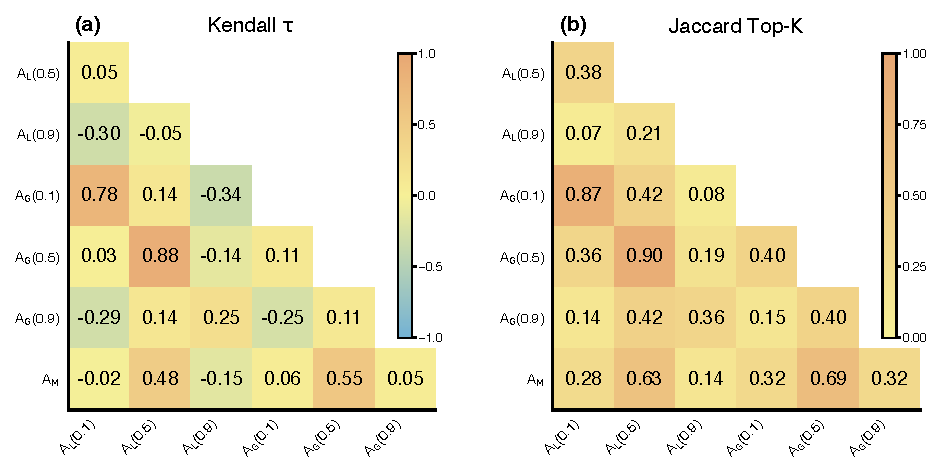
\includegraphics[width=\textwidth]{figures/policy_compliance_operator_agreement.pdf}
    \caption{Pairwise agreement among the seven aggregation configurations
considered in Experiment~01 ($N=1000$, $K=100$, $1000$ Monte Carlo
replications). The configurations are $A_L$ and $A_G$ at
$\lambda\in\{0.10,0.50,0.90\}$ and $A_M$. Each cell reports the Monte Carlo
mean of the corresponding pairwise statistic across replications.
(\textbf{a})~Kendall's $\tau_b$ between the aggregated-score rankings.
(\textbf{b})~Jaccard similarity between the corresponding Top-$K$ sets.
Higher values indicate greater agreement; the diagonal is omitted because
self-comparisons are identically equal to one.}
\label{fig:policy-operator-agreement}
\end{figure}

The experiment also reveals that the aggregation semantics affect more than
the treatment of explicit vetoes. Figure~\ref{fig:policy-operator-agreement}
compares the resulting prioritizations across seven representative
configurations: $A_L$ and $A_G$ at
$\lambda\in\{0.10,0.50,0.90\}$, together with $A_M$. Kendall's
$\tau_b$ measures agreement between their induced score rankings, whereas
Jaccard similarity measures the overlap between the corresponding Top-$K$
sets. Thus, the two statistics distinguish changes in the overall ordering
from changes in the actual alternatives selected for intervention.

The pairwise results show that aggregation semantics can produce similar
decisions when the predictive and contextual contributions are balanced, but
the agreement can decrease substantially when a highly predictive weight is
combined with a compensatory operator. For example, $A_L(0.50)$ and
$A_G(0.50)$ retain a relatively high mean rank agreement
($\tau_b>0.88$), whereas the comparison between $A_L(0.90)$ and
$A_G(0.10)$ yields mean $\tau_b<0$ and a Jaccard overlap below $0.15$.
The latter case illustrates a stronger form of semantic divergence: the two
systems can assign substantially different priorities to the same
alternatives and consequently select largely different Top-$K$ sets. This
divergence should not be interpreted as evidence that one operator is
generally superior. Rather, it shows that the choice of aggregation
semantics is itself a consequential modelling decision in CADEMAS-ML.

These observations are consistent with Theorem~\ref{thm:veto-preservation}
and Corollary~\ref{cor:topk-exclusion}. The theorem establishes the
score-level consequence of zero absorption, while the corollary identifies
the additional population-level condition under which this property becomes
Top-$K$ exclusion. The simulation shows the complementary case for the
linear operator: because it is compensatory and does not satisfy zero
absorption, the theory provides no exclusion guarantee, and the actual
population distribution determines when vetoed alternatives become
competitive. The dense sweep therefore quantifies a population-level
effect that cannot be inferred from the operator definition alone.

Overall, the experiment shows two distinct consequences of aggregation
semantics. Zero-absorbing operators preserve contextual vetoes under the
conditions of Corollary~\ref{cor:topk-exclusion}, whereas the compensatory
linear operator can trade contextual admissibility against predictive
evidence as $\lambda$ increases. At the same time, the Kendall and Jaccard
results demonstrate that these semantic differences propagate to the final
prioritization itself. The aggregation operator is therefore not merely a
technical implementation detail: it can determine both whether excluded
alternatives remain excluded and which alternatives ultimately constitute
the Top-$K$ decision set.

\subsection{Sensitivity Analysis}
\label{subsec:sensitivity-analysis}

The second experiment examines how uncertainty in the predictive pathway
propagates to the prioritization produced by CADEMAS-ML, addressing
\textit{RQ3} and \textit{RQ4}. We focus on perturbations of the predictive
score because $R$ represents the output of an ADM or predictive model and
can therefore be affected by estimation error. For the three aggregation
operators considered here, the same analysis applies to contextual
perturbations by exchanging $R$ and $Q$ and, for the linear and geometric
operators, replacing $\lambda$ by $1-\lambda$. We therefore use noise on
$R$ as the representative uncertainty channel rather than duplicating an
analytically symmetric experiment on $Q$.

For each of the $1000$ Monte Carlo populations, the predictive scores are
perturbed according to Eq.~(\ref{eq:r-noise}), with
$\sigma_R\in\{0.05,0.10,0.20\}$.
The contextual scores remain unchanged, including the $20\%$ of cases with
$Q_i=0$. We evaluate the seven ranking configurations used throughout the
experiments: $A_L$ and $A_G$ at
$\lambda\in\{0.10,0.50,0.90\}$, together with $A_M$. These values provide
low, intermediate, and high predictive weighting for the two
$\lambda$-dependent operators, while $A_M$ serves as the
$\lambda$-independent reference. For each configuration, we record the
policy violation rate $V$ and compare the noisy ranking with the clean
ranking obtained from the same population before perturbation, using
Kendall's $\tau_b$ and the Top-$K$ Jaccard similarity. We also compare the
seven configurations with one another under the same noisy realization,
which allows us to distinguish loss of stability relative to the clean
ranking from changes in the agreement between aggregation semantics.

Figure~\ref{fig:sensitivity-r-noise-overview} first illustrates how the
perturbation changes the underlying population. Panels~(a)--(c) show the
same Monte Carlo population at increasing noise levels. Since $Q$ is fixed,
the perturbation acts horizontally in the $(R,Q)$ plane. The vetoed cases
therefore remain on the $Q=0$ boundary, whereas non-vetoed alternatives are
increasingly dispersed in the predictive dimension. At the largest noise
level, the clipping operation also becomes visible through the accumulation
of observations at the boundaries of the admissible range. This is
important for interpreting the subsequent ranking results: the perturbation
is not equivalent to an unconstrained Gaussian displacement, but to noisy
scores projected back onto $[0,1]$.

\begin{figure}[H]
\centering
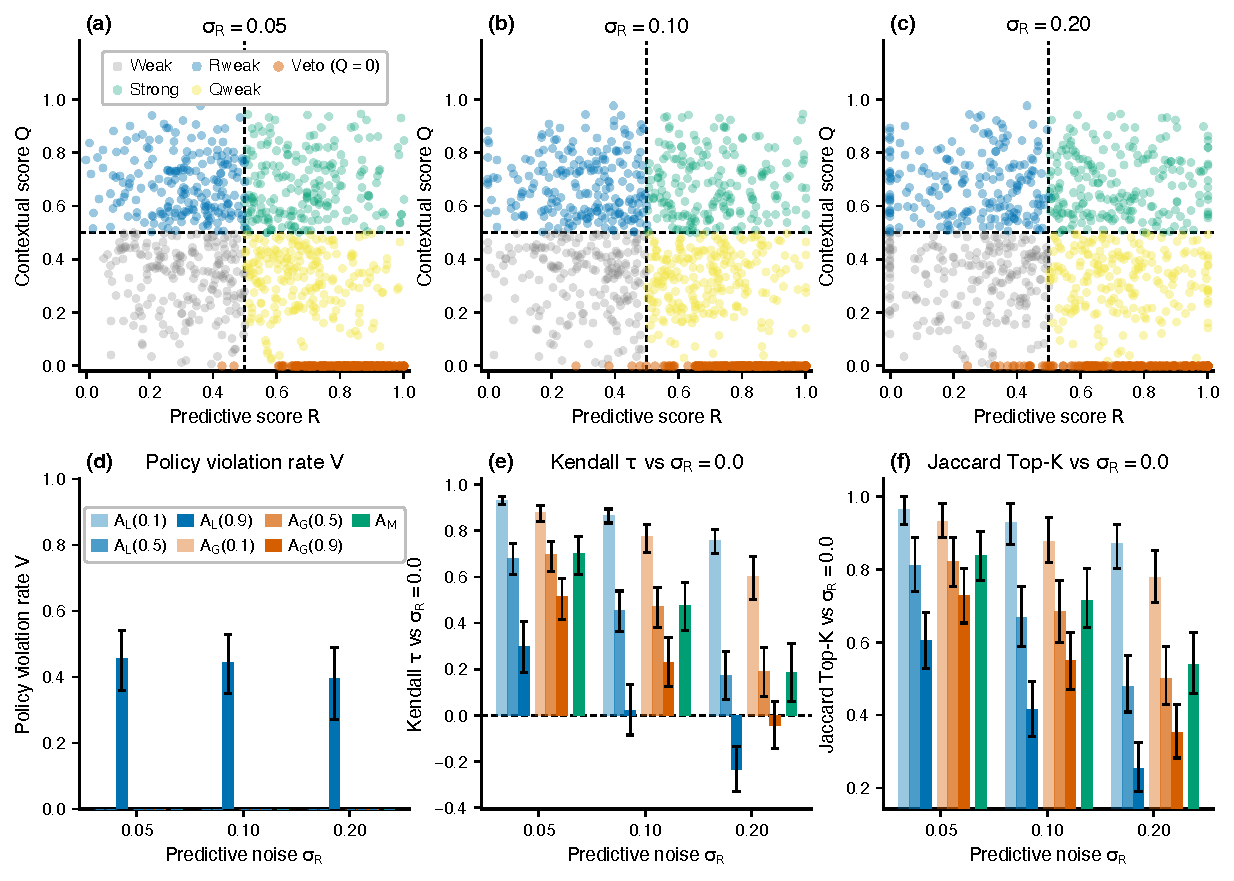
\includegraphics[width=\textwidth]{figures/sensitivity_r_noise_overview.pdf}
\caption{Sensitivity to predictive-score perturbations. Panels (a)--(c)
show one illustrative population at increasing noise levels. Panels
(d)--(f) summarize the corresponding Monte Carlo results for the seven
ranking configurations.}
\label{fig:sensitivity-r-noise-overview}
\end{figure}

The population-level consequences are shown in panels~(d)--(f). The first
pattern concerns policy compliance. The zero-absorbing operators
$A_G$ and $A_M$ retain $V=0$ across the tested noise levels, whereas noise
does not provide any additional protection for the compensatory linear
operator. In particular, the high-predictive configuration $A_L(0.90)$
continues to exhibit substantial violations at the larger noise levels.
This is consistent with Theorem~\ref{thm:veto-preservation}: perturbing
$R$ does not alter the fact that $A_G$ and $A_M$ map a true contextual veto
$Q_i=0$ to zero. Since the population satisfies the supply condition of
Corollary~\ref{cor:topk-exclusion}, this score-level property continues to
exclude vetoed alternatives from the Top-$K$ set.

The second pattern is the loss of agreement with the clean ranking. At
$\sigma_R=0.05$, the perturbation produces a moderate degradation for most
configurations, but the effect becomes much stronger as the noise
increases. The degradation is also operator-dependent: configurations that
give greater weight to $R$ are generally more sensitive, particularly for
the linear operator. At $\sigma_R=0.20$, for example, the mean Kendall
correlation for $A_L(0.90)$ falls to approximately $-0.24$, while its
Top-$K$ Jaccard similarity is only about $0.25$. Thus, at sufficiently
large perturbations, the noisy prioritization can differ substantially
from the clean one, both in the global ordering and in the actual set of
selected alternatives. The stronger decrease in Jaccard than in Kendall's
$\tau_b$ indicates that the instability is particularly consequential near
the Top-$K$ boundary.

The comparison between operators under the same noisy realizations is
shown in Figure~\ref{fig:sensitivity-operator-agreement}. The heatmaps
provide a complementary view of the previous analysis: rather than asking
whether each configuration remains close to its own clean ranking, they
ask whether different aggregation semantics continue to select similar
alternatives when exposed to the same uncertain predictive scores.
Agreement generally decreases as $\sigma_R$ increases, but the reduction
is not uniform across configurations. In particular, configurations with
different $\lambda$ values can diverge substantially, while configurations
with similar integration semantics remain more closely aligned. The
result therefore confirms that uncertainty does not erase the effect of
aggregation semantics; instead, it interacts with the way each operator
translates the perturbed evidence into prioritization scores.

\begin{figure}[H]
\centering
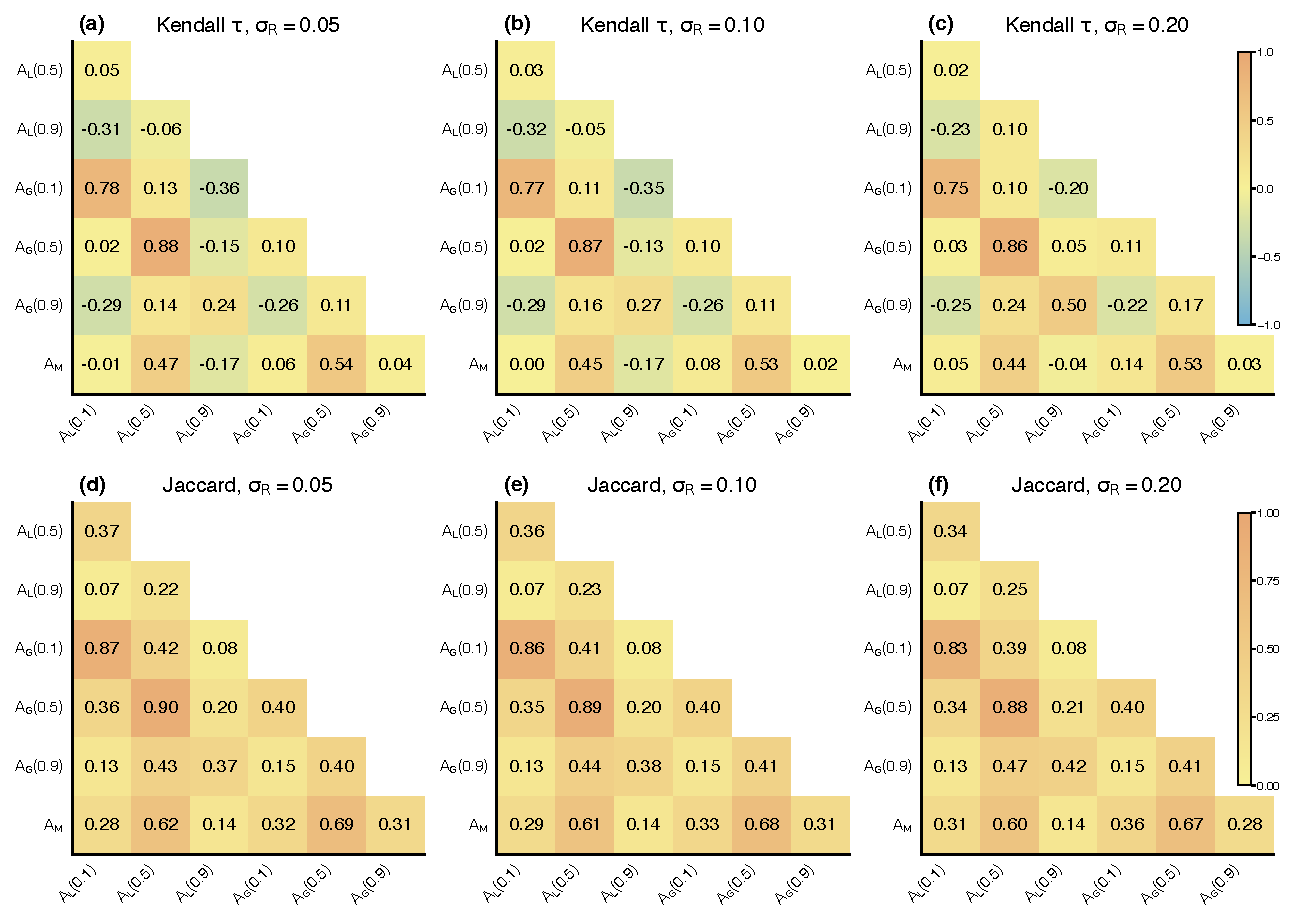
\includegraphics[width=\textwidth]{figures/sensitivity_operator_agreement.pdf}
\caption{Pairwise agreement among the seven ranking configurations under
shared predictive-score perturbations. The heatmaps report mean Kendall
$\tau_b$ and Top-$K$ Jaccard similarity across Monte Carlo replications.}
\label{fig:sensitivity-operator-agreement}
\end{figure}

Taken together, the experiment shows two distinct effects of predictive
uncertainty. It can alter the prioritization produced by all operators,
especially when predictive evidence receives high weight, but it does not
remove the structural distinction established by the theory. Zero
absorption protects the veto mechanism of $A_G$ and $A_M$, whereas the
linear operator remains compensatory and can therefore propagate
high predictive scores into contextually excluded alternatives. The
sensitivity analysis consequently complements the deterministic results of
the previous experiment: uncertainty changes the stability of the
resulting ranking, but it does not change the underlying aggregation
semantics that determine whether contextual vetoes are structurally
preserved.

\section{Employee Attrition Case Study} 
\label{sec:employee-attrition-case-study}
% R1-10
% Presentarlo como ilustración.
% No como validación independiente.

\subsection{Original CADEMAS-ML Application}

% Explicar origen de scores.

\subsection{Experimental Setup}

% R1-10
% Top-K.
% Empates.
% Context scores.
% Procedimiento.

\subsection{Results and Interpretation}

% R1-10
% Mostrar estabilidad para distintos K.

%%%%%%%%%%%%%%%%%%%%%%%%%%%%%%%%%%%%%%%%%%%%%%%%%%%%%%%%%%%%

\section{Discussion}

% R1-1, R1-8, R2-2

\subsection{Implications for Cooperative Automated Decision Making}

% Discusión conceptual.

\subsection{Relation to Fuzzy MCDM and Aggregation Theory}

% R1-1, R2-2
% Subsection MUY IMPORTANTE.
%
% Explicar explícitamente:
% - qué NO aporta el paper;
% - qué sí aporta.
%
% Distinguir:
% aggregation theory,
% fuzzy MCDM,
% CADEMAS.

\subsection{Limitations}

% R1-8, R1-10
% Limitar alcance de conclusiones.

%%%%%%%%%%%%%%%%%%%%%%%%%%%%%%%%%%%%%%%%%%%%%%%%%%%%%%%%%%%%

\section{Conclusions and Future Work}

% R1-8
% Moderar afirmaciones.
%
% No decir:
% "nonlinear operators are superior".
%
% Decir:
% "under the considered conditions".

% Futuro:
% OWA,
% Choquet,
% learned aggregation,
% dynamic policies.

%%%%%%%%%%%%%%%%%%%%%%%%%%%%%%%%%%%%%%%%%%
\authorcontributions{To be completed.}

\funding{This research was supported by the project ``Study, Analysis and Evaluation of Cooperative Automated Decision-Making Systems (CADEMAS)'', PID2023-146575NB-I00, funded by MCIU/AEI/I0.13039/501100011033 and by FSE+.}

\institutionalreview{Not applicable.}

\informedconsent{Not applicable.}

\dataavailability{To be completed.}

\acknowledgments{Mariia Godz has a pre-doctoral research contract associated with the project ``Study, Analysis and Evaluation of Cooperative Automated Decision-Making Systems (CADEMAS)'', PID2023-146575NB-I00, funded by MCIU/AEI/I0.13039/501100011033 and by FSE+.}

\conflictsofinterest{The authors declare no conflicts of interest.}

%%%%%%%%%%%%%%%%%%%%%%%%%%%%%%%%%%%%%%%%%%
\begin{adjustwidth}{-\extralength}{0cm}
\reftitle{References}
%\bibliography{biblio}

\begin{thebibliography}{999}

\bibitem[Teng and Tan(2008)]{TengTan2008}
Teng, T.H.; Tan, A.H.
\newblock Cognitive Agents Integrating Rules and Reinforcement Learning for Context-Aware Decision Support.
\newblock In Proceedings of the Proceedings of the 2008 IEEE/WIC/ACM International Conference on Web Intelligence and Intelligent Agent Technology,  2008, pp. 318--321.
\newblock {\url{https://doi.org/10.1109/WIIAT.2008.163}}.

\bibitem[Yao and Kumar(2012)]{YaoKumar2012}
Yao, W.; Kumar, A.
\newblock Integrating Clinical Pathways into {CDSS} Using Context and Rules: A Case Study in Heart Disease.
\newblock In Proceedings of the Proceedings of the 2nd ACM SIGHIT International Health Informatics Symposium,  2012, pp. 267--276.
\newblock {\url{https://doi.org/10.1145/2110363.2110431}}.

\bibitem[Abu-Rasheed et~al.(2024)Abu-Rasheed, Abdulsalam, Weber, and Fathi]{AbuRasheed2024}
Abu-Rasheed, H.; Abdulsalam, M.; Weber, C.; Fathi, M.
\newblock Supporting Student Decisions on Learning Recommendations: An {LLM}-Based Chatbot with Knowledge Graph Contextualization for Conversational Explainability and Mentoring.
\newblock {\em Frontiers in Artificial Intelligence} {\bf 2024}.
\newblock {\url{https://doi.org/10.35542/osf.io/ervym}}.

\bibitem[Casado and Fernandez(2025)]{Casado2025Governance}
Casado, D.F.; Fernandez, R.P.
\newblock A Governance-Aware Methodological Framework for Cognitive {AI} Integration in Marine {CAD}: A Conceptual Pipe Routing Use Case.
\newblock {\em Journal of Marine Science and Engineering} {\bf 2025}, {\em 14},~1352.
\newblock {\url{https://doi.org/10.3390/jmse14011352}}.

\bibitem[Cronholm and G{\"o}bel(2022)]{CronholmGoebel2022}
Cronholm, S.; G{\"o}bel, H.
\newblock Design Principles for Human-Centred {AI}.
\newblock In Proceedings of the ECIS 2022 Research Papers,  2022.
\newblock Research paper 32.

\bibitem[Fanfani et~al.(2025)Fanfani, Palesi, and Nesi]{Fanfani2025Human}
Fanfani, M.; Palesi, L.A.I.; Nesi, P.
\newblock Human-Centered {AI} for Decision Support Systems: A Systematic Review of Application Domains, Architecture Designs, Current Trends and Future Directions.
\newblock {\em Big Data and Cognitive Computing} {\bf 2025}, {\em 10},~186.
\newblock {\url{https://doi.org/10.3390/bdcc10060186}}.

\bibitem[Smirnov et~al.(2021)Smirnov, Levashova, Ponomarev, and Shilov]{Smirnov2021Methodology}
Smirnov, A.V.; Levashova, T.; Ponomarev, A.; Shilov, N.
\newblock Methodology for Multi-Aspect Ontology Development: Ontology for Decision Support Based on Human-Machine Collective Intelligence.
\newblock {\em IEEE Access} {\bf 2021}, {\em 9},~130721--130739.
\newblock {\url{https://doi.org/10.1109/ACCESS.2021.3116870}}.

\bibitem[Marot et~al.(2022)Marot, Kelly, Naglic, Barbesant, and Cremer]{Marot2022Perspectives}
Marot, A.; Kelly, A.; Naglic, M.; Barbesant, V.; Cremer, J.L.
\newblock Perspectives on Future Power System Control Centers for Energy Transition.
\newblock {\em Journal of Modern Power Systems and Clean Energy} {\bf 2022}, {\em 10},~328--344.
\newblock {\url{https://doi.org/10.35833/mpce.2021.000673}}.

\bibitem[Novoa-Hernández et~al.(2026)Novoa-Hernández, Pelta, Godz, Verdegay, and Buendia-Carrillo]{NovoaHernandez2026}
Novoa-Hernández, P.; Pelta, D.; Godz, M.; Verdegay, J.; Buendia-Carrillo, D.
\newblock {CADEMAS} – A Framework for Cooperative Automated Decision-Making Systems.
\newblock In Proceedings of the Proceedings of the 2026 IEEE Conference on Artificial Intelligence (CAI),  2026, pp. 756--761.
\newblock {\url{https://doi.org/10.1109/CAI68641.2026.11536392}}.

\bibitem[Godz et~al.(2026)Godz, Novoa-Hernández, and Pelta]{Godz2026}
Godz, M.; Novoa-Hernández, P.; Pelta, D.
\newblock A Cooperative and Context-Aware Approach for Employee Attrition Prevention. In {\em Information Processing and Management of Uncertainty in Knowledge-Based Systems}; Springer Nature Switzerland,  2026; pp. 203--217.
\newblock {\url{https://doi.org/10.1007/978-3-032-29000-7_15}}.

\bibitem[Yager(1988)]{Yager1988}
Yager, R.
\newblock On Ordered Weighted Averaging Aggregation Operators in Multicriteria Decisionmaking.
\newblock {\em IEEE Transactions on Systems, Man, and Cybernetics} {\bf 1988}, {\em 18},~183--190.
\newblock {\url{https://doi.org/10.1109/21.87068}}.

\bibitem[Yager(2005)]{Yager2005}
Yager, R.R.
\newblock Extending Multicriteria Decision Making by Mixing t-Norms and {OWA} Operators.
\newblock {\em International Journal of Intelligent Systems} {\bf 2005}, {\em 20},~453--474.
\newblock {\url{https://doi.org/10.1002/int.20075}}.

\bibitem[Mardani et~al.(2018)Mardani, Nilashi, Zavadskas, Awang, Zare, and Jamal]{Mardani2018}
Mardani, A.; Nilashi, M.; Zavadskas, E.K.; Awang, S.; Zare, H.; Jamal, N.M.
\newblock Decision making methods based on fuzzy aggregation operators: Three decades review from 1986 to 2017.
\newblock {\em International Journal of Information Technology \& Decision Making} {\bf 2018}, {\em 17},~391--466.
\newblock {\url{https://doi.org/10.1142/S021962201830001X}}.

\bibitem[Csisz{\'a}r(2021)]{Csiszar2021}
Csisz{\'a}r, O.
\newblock Ordered Weighted Averaging Operators: A Short Review.
\newblock {\em IEEE Systems, Man, and Cybernetics Magazine} {\bf 2021}, {\em 7},~4--12.
\newblock {\url{https://doi.org/10.1109/MSMC.2020.3036378}}.

\bibitem[del Moral et~al.(2017)del Moral, Chiclana, Tapia~Garc{\'i}a, and Herrera-Viedma]{MoralEtAl2017}
del Moral, M.J.; Chiclana, F.; Tapia~Garc{\'i}a, J.M.; Herrera-Viedma, E.
\newblock An Analysis on Consensus Measures in Group Decision Making.
\newblock In Proceedings of the Proceedings of the 2017 4th International Conference on Control, Decision and Information Technologies (CoDIT),  2017, pp. 0262--0267.
\newblock {\url{https://doi.org/10.1109/CoDIT.2017.8102605}}.

\bibitem[Trillo et~al.(2023)Trillo, Cabrerizo, del Moral, Morente-Molinera, Tapia, and Herrera-Viedma]{TrilloEtAl2023}
Trillo, J.R.; Cabrerizo, F.J.; del Moral, M.J.; Morente-Molinera, J.A.; Tapia, J.M.; Herrera-Viedma, E.
\newblock A Consensus-Based Multi-Criteria Group Decision-Making Method Based on an Aggregated Operator Customised by Experts.
\newblock In Proceedings of the Proceedings of the 2023 9th International Conference on Control, Decision and Information Technologies (CoDIT),  2023.
\newblock {\url{https://doi.org/10.1109/CoDIT58514.2023.10284209}}.

\bibitem[Yang et~al.(2022)Yang, Lin, Fu, and Luo]{Yang2022Tolerance}
Yang, Y.W.; Lin, J.K.; Fu, Y.; Luo, Y.
\newblock Tolerance Framework for Robust Group Multiple Criteria Decision Making.
\newblock {\em Expert Systems with Applications} {\bf 2022}, {\em 204},~117430.
\newblock {\url{https://doi.org/10.1016/j.eswa.2022.118208}}.

\bibitem[Liao et~al.(2023)Liao, Liao, and Zhang]{Liao2023Contextual}
Liao, Z.; Liao, H.; Zhang, X.
\newblock A Contextual {Choquet} Integral-Based Preference Learning Model Considering Both Criteria Interactions and the Compromise Effects of Decision-Makers.
\newblock {\em Expert Systems with Applications} {\bf 2023}, {\em 213},~118977.
\newblock {\url{https://doi.org/10.1016/j.eswa.2022.118977}}.

\bibitem[Stroppiana et~al.(2022)Stroppiana, Boschetti, Brivio, Manfron, and Antoninetti]{Stroppiana2022Explainable}
Stroppiana, D.; Boschetti, M.; Brivio, P.A.; Manfron, G.; Antoninetti, M.
\newblock Explainable Multi-Criteria Data-Driven Environmental Status Assessment from Remote Sensing.
\newblock In Proceedings of the Proceedings of the IEEE MELECON 2022,  2022.
\newblock {\url{https://doi.org/10.1109/MELECON53508.2022.9842919}}.

\bibitem[Alcantud(2023)]{Alcantud2023Multi}
Alcantud, J.C.R.
\newblock Multi-Attribute Group Decision-Making Based on Intuitionistic Fuzzy Aggregation Operators Defined by Weighted Geometric Means.
\newblock {\em Granular Computing} {\bf 2023}, {\em 8},~1857--1866.
\newblock {\url{https://doi.org/10.1007/s41066-023-00406-w}}.

\bibitem[Merkert et~al.(2015)Merkert, Mueller, and Hubl]{MerkertEtAl2015}
Merkert, J.; Mueller, M.; Hubl, M.
\newblock A Survey of the Application of Machine Learning in Decision Support Systems.
\newblock In Proceedings of the Proceedings of the 23rd European Conference on Information Systems (ECIS),  2015.
\newblock {\url{https://doi.org/10.18151/7217429}}.

\bibitem[Pérez-Cañedo et~al.(2023)Pérez-Cañedo, Porras, Pelta, and Verdegay]{PerezCanedo2022}
Pérez-Cañedo, B.; Porras, C.; Pelta, D.; Verdegay, J.
\newblock Modeling Contexts as Fuzzy Propositions in Optimization Problems.
\newblock {\em {IEEE} Transactions on Fuzzy Systems} {\bf 2023}, {\em 31},~1474--1483.
\newblock {\url{https://doi.org/10.1109/tfuzz.2022.3203786}}.

\bibitem[P{\'e}rez-Ca{\~n}edo et~al.(2024)P{\'e}rez-Ca{\~n}edo, Novoa-Hern{\'a}ndez, Porras, Pelta, and Verdegay]{PerezCanedo2024}
P{\'e}rez-Ca{\~n}edo, B.; Novoa-Hern{\'a}ndez, P.; Porras, C.; Pelta, D.; Verdegay, J.
\newblock Contextual analysis of solutions in a tourist trip design problem: A fuzzy logic-based approach.
\newblock {\em Applied Soft Computing} {\bf 2024}, {\em 154},~111351.
\newblock {\url{https://doi.org/10.1016/j.asoc.2024.111351}}.

\end{thebibliography}
\end{adjustwidth}
\PublishersNote{}

\end{document}
